

\begin{frame}{Distributed SHE}

  \begin{center}
    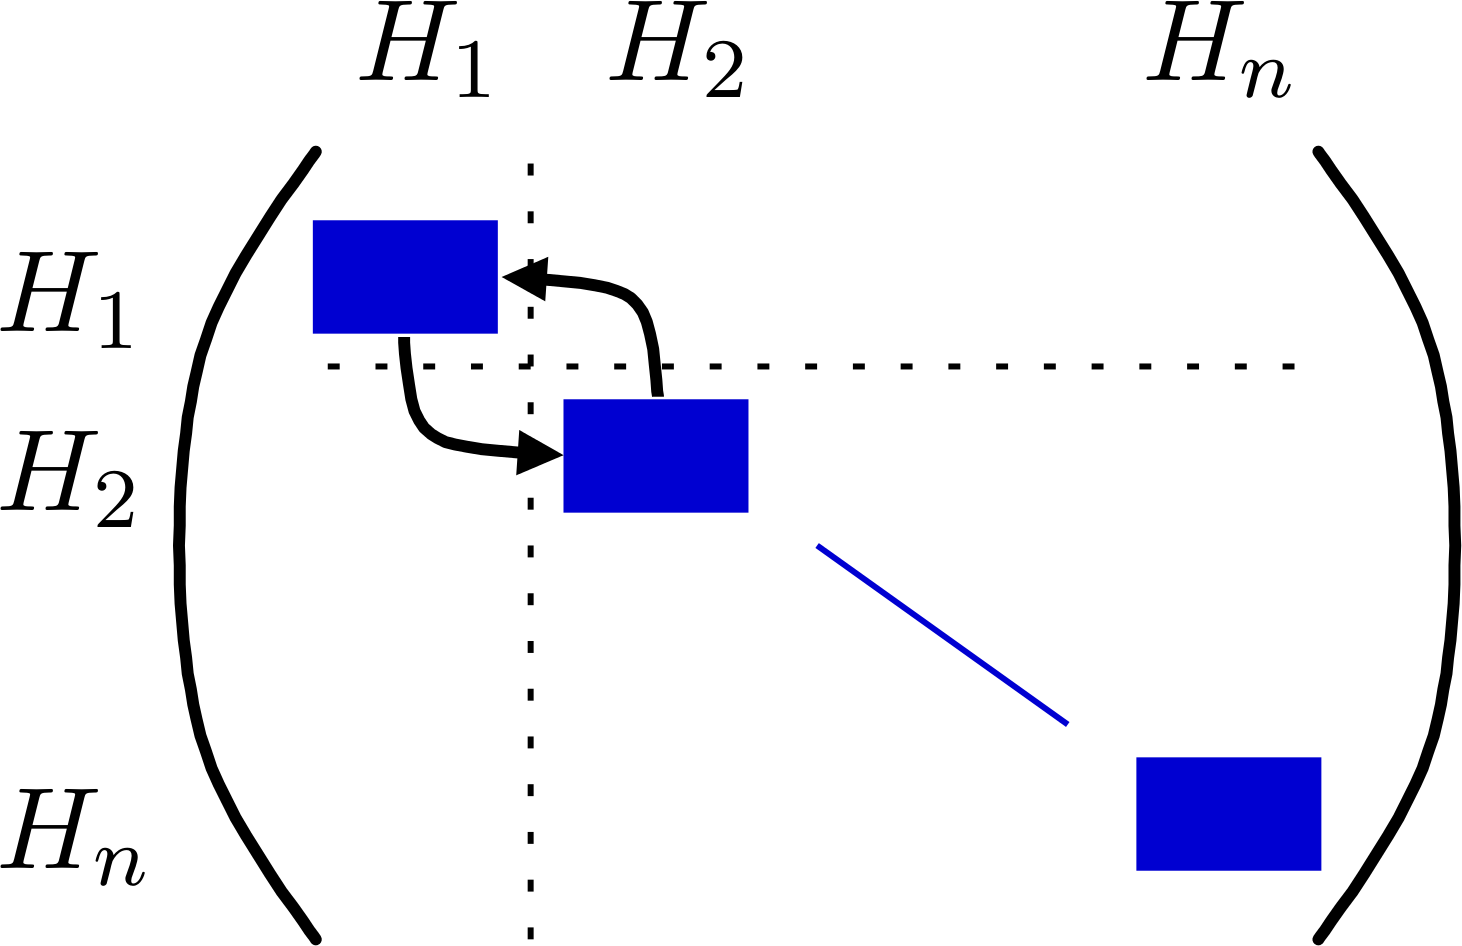
\includegraphics[width=0.45\textwidth]{matrix-structure-2}
  \end{center}

  %\pause
  
  \begin{block}{Blueprint}
   \begin{itemize}
    \item Keep block-Jacobi based on total energies
    \item Map total energies to MPI ranks
    \item Requires fine-grained parallel preconditioner per block
   \end{itemize}
  \end{block}
  
\end{frame}


\begin{frame}{Parallel ILU}

  \begin{block}{General}
   \begin{itemize}
    \item Approximate factorization $\mathbf{A} \approx \mathbf{L} \mathbf{U}$
    \item Proposed by Chow and Patel (SISC, vol.~37(2)) for CPUs and MICs
    \item Available in ViennaCL for CUDA, OpenCL, OpenMP
   \end{itemize}
  \end{block}
  
  %\pause

  \begin{block}{Preconditioner Setup}
   \begin{itemize}
    \item Nonlinear parallel sweeps to obtain $l_{ij}$ and $u_{ij}$
    \item Massively parallel (one thread per row)
   \end{itemize}
  \end{block}

  %\pause
  
  \begin{block}{Preconditioner Application}
   \begin{itemize}
    \item Truncated Neumann series:
     \begin{align*} \mathbf{L}^{-1} \approx \sum_{k=0}^K (\mathbf{I} - \mathbf{L})^k, \quad \mathbf{U}^{-1} \approx \sum_{k=0}^K (\mathbf{I} - \mathbf{U})^k \end{align*}
    \item Exact triangular solves not necessary
   \end{itemize}
  \end{block}

\end{frame}


\begin{frame}{Parallel ILU}

  \begin{center}
    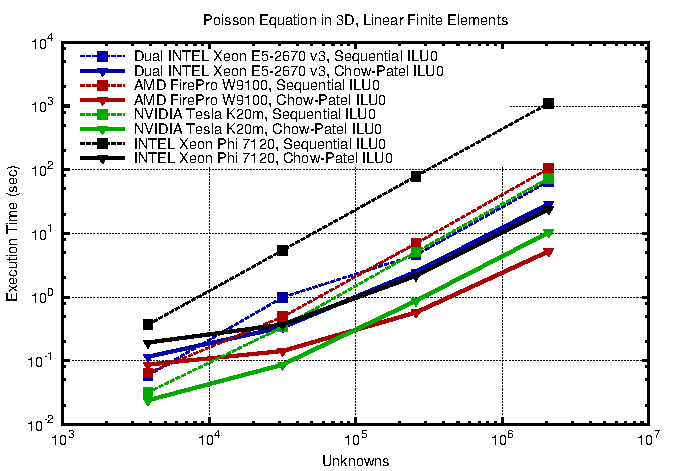
\includegraphics[width=0.95\textwidth]{ilu-3d}
  \end{center}
\end{frame}


\begin{frame}{Preconditioner Evaluation}

  \begin{block}{Resolution}
   \begin{itemize}
    \item Total energy spacing: approx. $10$ meV 
    \item Thus: Hundred MPI ranks per eV (slight load imbalance)
    \item Typical minimum range: $3$-$5$ eV
   \end{itemize}
  \end{block}

  %\pause
  
  \begin{block}{Granularity}
   \begin{itemize}
    \item Fine-grained: One thread per matrix row on each MPI rank
    \item Coarse-grained: One run per voltage bias
   \end{itemize}
  \end{block}

  %\pause
  
  \begin{block}{Evaluation}
   \begin{itemize}
    \item Preconditioner sufficient for typical TCAD workloads
    \item Ready for upcoming HPC hardware
    \item Spatial domain decomposition required for strong scaling limit
   \end{itemize}
  \end{block}

\end{frame}

\begin{frame}{Preconditioner Alternatives}

  \begin{center}
    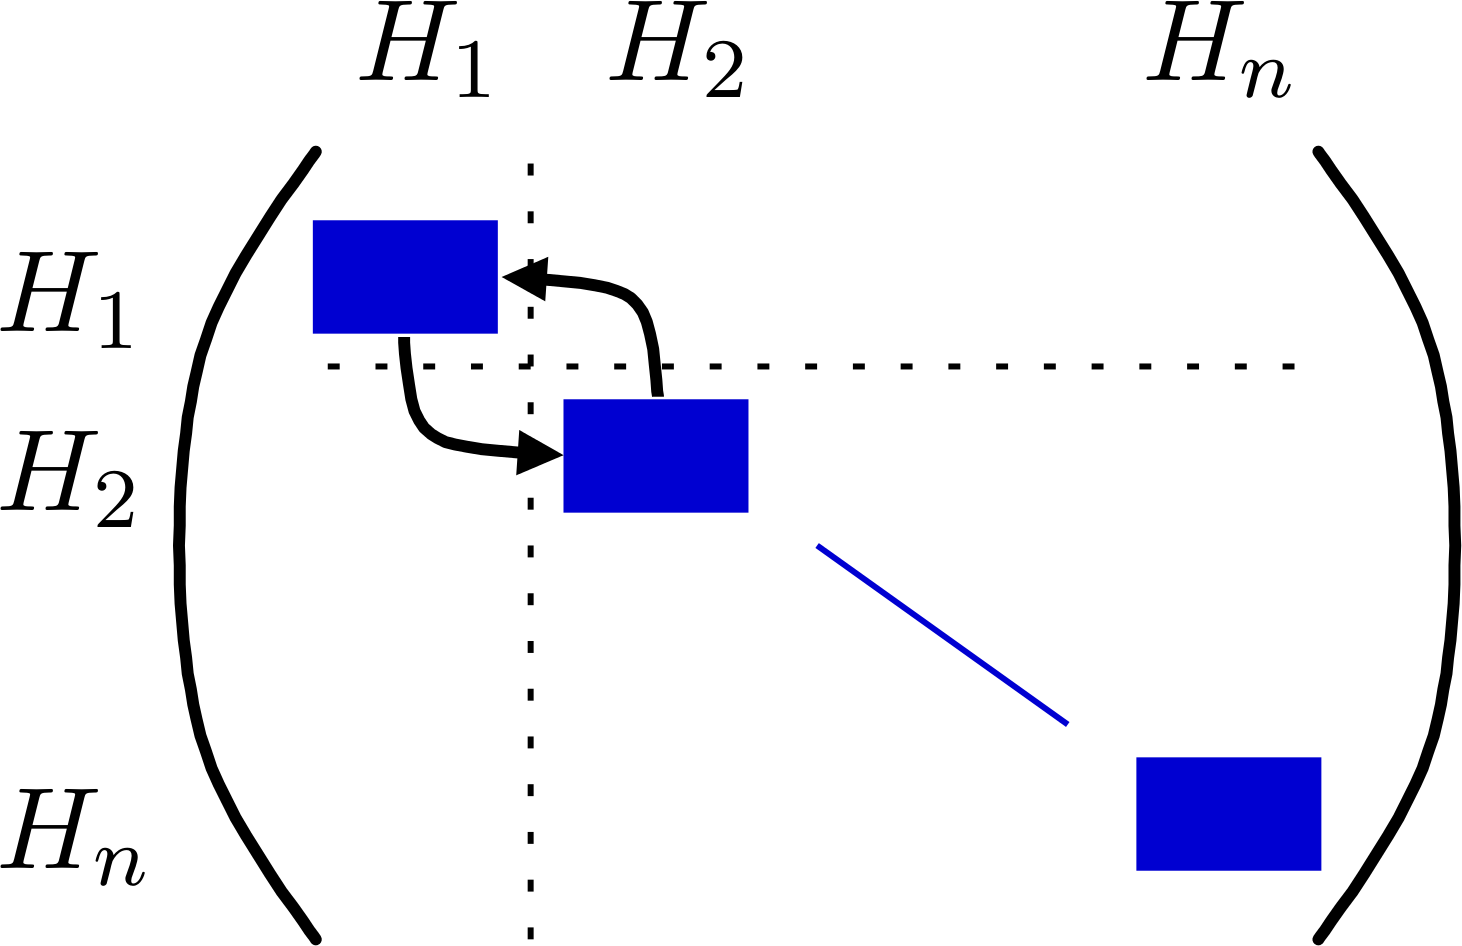
\includegraphics[width=0.4\textwidth]{matrix-structure-2}
  \end{center}

  \begin{block}{Other Shared Memory Preconditioners}
   \begin{itemize}
    \item Algebraic multigrid?
    \item Polynomial preconditioners?
   \end{itemize}
  \end{block}

  %\pause
  
  \begin{block}{Block-Diagonal Inversion}
   \begin{itemize}
    \item Additive Schwarz (no overlap)
    \item Sparse direct solver for each block?
   \end{itemize}
  \end{block}

\end{frame}


\begin{frame}{Parallel AMG}
  \begin{center}
    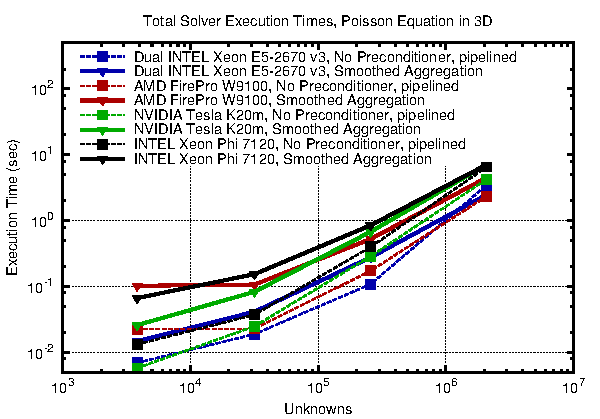
\includegraphics[width=0.95\textwidth]{amg-vs-pure-full-3d}
  \end{center}
\end{frame}

